\documentclass[fleqn,10pt]{wlscirep}
\usepackage[utf8]{inputenc}
\usepackage[T1]{fontenc}
\usepackage{amsmath,amssymb,amsfonts}
\usepackage{graphicx}
\usepackage{textcomp}
\usepackage{algorithm}
\usepackage{algpseudocode}
\usepackage{float}
\usepackage{booktabs}        % for \toprule \midrule \bottomrule
\usepackage{threeparttable}  % for \tnote and tablenotes
\usepackage{array}           % for p{} column type
\usepackage{longtable}
\usepackage{xcolor}
\usepackage{url}
\setlength{\emergencystretch}{2em}

% Clean publication version. Revision commands are retained structurally so
% that this source remains text-identical to the highlighted manuscript, but
% all content is rendered in normal black.
\definecolor{revisionblue}{RGB}{0,0,0}
\newcommand{\rev}[1]{{\color{revisionblue}#1}}
\newenvironment{revision}{\color{revisionblue}}{}

% Numerical values are generated directly from saved revision experiment
% artifacts.
\IfFileExists{revision_results.tex}{\input{revision_results.tex}}{
  \newcommand{\METRMAE}{TBD}
  \newcommand{\METRMAESD}{TBD}
  \newcommand{\PEMSMAE}{TBD}
  \newcommand{\PEMSMAESD}{TBD}
  \newcommand{\METRAttentionMAE}{TBD}
  \newcommand{\METRAttentionMAESD}{TBD}
  \newcommand{\PEMSAttentionMAE}{TBD}
  \newcommand{\PEMSAttentionMAESD}{TBD}
  \newcommand{\AttentionDelta}{TBD}
  \newcommand{\PEMSAttentionDelta}{TBD}
  \newcommand{\GammaBest}{TBD}
  \newcommand{\GraphStability}{TBD}
  \newcommand{\PEMSGraphStability}{TBD}
  \newcommand{\METRTopTenStability}{TBD}
  \newcommand{\PEMSTopTenStability}{TBD}
}
\title{ASTAF-R: An Ablation-Guided Spatio-Temporal Framework for Multi-Horizon Traffic Prediction}

\author[1,+]{Shishir Singh Chauhan}
\author[2,+]{Puneet Nema}
\author[3,+]{Gunjan Chhabra}
\author[1,*]{Ankur Pandey}
\author[1,+]{Surbhi Syal}
\affil[1]{Manipal University Jaipur, Department of Computer Science and Engineering, Jaipur, 303007, INDIA}
\affil[2]{Department of Computer Science and Engineering, Lakshmi Narain College of Technology, Bhopal, MP, INDIA}
\affil[3]{Department of computer science and engineering, School of science and technology, Swami Rama Himalayan University, Dehradun, Uttarakhand, INDIA}

\affil[*]{ankur.pandey@jaipur.manipal.edu}

\affil[+]{these authors contributed equally to this work}

\setlength{\textfloatsep}{6pt}
\setlength{\floatsep}{6pt}
\setlength{\intextsep}{6pt}

\keywords{Traffic forecasting, Intelligent transportation systems, Spatio-temporal learning, Graph neural networks, Adaptive graph learning, Ablation-guided refinement, Multi-horizon prediction, Time series decomposition}

\begin{abstract}
{\color{revisionblue}
Reliable traffic forecasting comparisons require architectural decisions to be
separated from final test evaluation and all models to share the same data
pipeline. ASTAF-R is an ablation-guided deterministic framework that combines
causal multi-scale temporal encoding, residual signal decomposition, sparse
graph propagation, residual spatial attention, and last-observation residual
decoding. Candidate variants were selected using validation MAE only, after
which the chosen configuration and eight compact common-code comparison models
were evaluated once on held-out test periods from METR-LA and PeMS-BAY. Raw
timelines were divided chronologically before stride-one 12-to-12 windows were
formed, preventing observations from crossing split boundaries. Across seeds
11, 22, and 33, ASTAF-R obtained 2.995$\pm$0.008 mph
MAE on METR-LA and 1.542$\pm$0.001 mph on PeMS-BAY.
The strongest compact comparison, STID-style, obtained
3.377$\pm$0.011 and
1.709$\pm$0.003 mph, respectively.
Calendar-day block bootstrap intervals remained below zero for ASTAF-R minus
each comparison model, while seed-level dispersion and resource measurements
are reported explicitly. A post-training graph audit found identical uniform
top-40 supports across seeds because the graph-source and graph-target
parameters converged to zero; consequently, the experiments support sparse
graph propagation but not a claim of recovered or seed-robust adaptive
topology. The evaluation is limited to two regularly sampled California
freeway-speed datasets and compact local baseline implementations. The results
therefore establish reproducible performance under this controlled protocol,
not universal or official state-of-the-art superiority.
}
\end{abstract}

\begin{document}
\flushbottom
\maketitle
% * <john.hammersley@gmail.com> 2015-02-09T12:07:31.197Z:
%
%  Click the title above to edit the author information and abstract
%
\thispagestyle{empty}



\section{Introduction}
\label{sec:intro}
Traffic-speed forecasting supports congestion warning, route guidance,
incident management, and network control. The task is difficult because road
measurements combine short-lived transitions, recurring daily structure,
spatial dependence, missing observations, and non-stationary disturbances.
Modern systems commonly assemble temporal convolutions, graph propagation,
attention, and signal decomposition in one architecture. Each component is
plausible, but adding plausible components does not by itself establish that
they improve held-out forecasting performance.

ASTAF-R treats architecture construction as an empirical selection problem.
The starting components are tested through validation-only ablations, and the
resulting configuration is frozen before the test set is evaluated. This
distinction matters because repeated test-guided refinement can produce an
optimistically biased comparison even when every individual run uses a
chronological split. The present protocol therefore separates candidate
selection, locked testing, and diagnostic analysis.

The input at each forecast origin contains 12 five-minute speed observations
from every sensor, and the model predicts the next 12 observations. METR-LA
contains 207 sensors and 34,272 time points; PeMS-BAY contains 325 sensors and
52,105 time points. In both cases, the raw timeline is divided into contiguous
70\%, 10\%, and 20\% segments before any windows are generated. This ordering
prevents the input or target observations of a window in one split from being
reused by a window in another split.

The comparison is intentionally controlled. Persistence and compact
STID-, DCRNN-, STGCN-, Transformer-, Graph WaveNet-, AGCRN-, and ASTAF-style
models use the same tensors, masks, optimizer family, stopping rule, and test
metrics. These implementations are useful common-code controls, but they are
not official repository reproductions or claims about the best published
configuration of each named method.

The main contributions are:
\begin{itemize}
\item a leakage-free raw-timeline split procedure with exact temporal boundary
records for two public traffic datasets;
\item validation-only selection followed by locked three-seed testing, with
seed-aware and calendar-day-block uncertainty analyses;
\item a deterministic ASTAF-R implementation combining temporal, decomposition,
sparse graph, residual-attention, and residual-decoder components;
\item transparent sensitivity and graph diagnostics, including evidence that
the learned graph parameters collapse to a uniform sparse support in the
selected runs; and
\item complete code, configurations, random seeds, run metadata, prediction
archives, and environment information for independent reproduction.
\end{itemize}

The remainder of the paper is organized as follows. Section~\ref{sec:related}
reviews statistical, recurrent, convolutional, graph, attention, decomposition,
and multi-scale forecasting methods. Section~\ref{sec:problem} defines the
multi-horizon task and metrics. Section~\ref{sec:data} describes both datasets,
preprocessing, and exploratory dependencies. Section~\ref{sec:method} specifies
ASTAF-R. Section~\ref{sec:setup} documents the leakage-free protocol, model
configurations, and computation environment. Section~\ref{sec:results} presents
the validation evidence, locked test results, statistical analyses, graph
diagnostics, and efficiency trade-offs. Section~\ref{sec:conclusion} states the
supported conclusions and limitations.

\section{Literature Review}
\label{sec:related}

Traffic forecasting has a long research history that spans classical
statistical methods, deep sequence models, convolutional architectures,
graph neural networks, and Transformer-based designs. This section
reviews each of these threads in the context of the design decisions
made in ASTAF-R, with particular attention to what is known about
the individual contributions of attention mechanisms, signal
decomposition, and adaptive graph topology learning.

% ------------------------------------------------------------
\subsection{Classical and Statistical Forecasting Methods}
% ------------------------------------------------------------

The earliest computational approaches to traffic forecasting were
rooted in classical time-series analysis. Autoregressive integrated
moving average (ARIMA) and its seasonal variant SARIMA modeled traffic
speed and flow as linear functions of their own past observations and
residual errors~\cite{box1970time}. These models remain valuable
in low-dimensional, single-sensor settings where the statistical
assumptions of stationarity and linearity approximately hold and where
interpretability of the model coefficients is required. Historical
average and exponential smoothing approaches provided simpler
alternatives with lower computational cost.

The fundamental limitation of classical methods in modern traffic
systems is their inability to scale. A road network with $N$ sensors
requires modeling $N$ separate time series, and the correlations
among those sensors, which carry important information about how
congestion propagates spatially, cannot be represented within a
univariate framework. Classical vector autoregression can model
joint dynamics across multiple series, but its parameter count grows
quadratically with $N$, making it computationally intractable for
the sensor counts typical of large urban networks. Non-linear
patterns, including sharp congestion onset and rapid clearance,
are also beyond the representational capacity of linear statistical
models. These limitations created the conditions for deep learning
to enter the problem.

% ------------------------------------------------------------
\subsection{Deep Recurrent and Convolutional Models}
% ------------------------------------------------------------

The first generation of deep learning approaches to traffic
forecasting replaced statistical models with recurrent neural
networks. Long short-term memory (LSTM) networks~\cite{hochreiter1997lstm}
addressed the vanishing gradient problem that limited standard
recurrent networks, enabling the learning of dependencies across
longer temporal windows. Gated recurrent units (GRU)~\cite{cho2014gru}
offered a computationally lighter alternative with comparable
representational capacity. Both architectures learn non-linear
sequential dependencies and can be stacked or combined with fully
connected layers to produce multi-step forecasts.

Convolutional architectures extended deep learning to the spatial
dimension in settings where traffic observations could be placed on
regular grids. ST-ResNet modeled citywide crowd flows as a sequence
of residual convolutional operations applied to grid-based
representations~\cite{zhang2017deepst}. Deep multi-view spatial-temporal
networks combined multiple temporal granularities within a single
convolutional architecture~\cite{yao2018deepmulti}. Spatio-temporal
meta learning frameworks further improved cross-region generalization
by learning shared feature representations~\cite{pan2019stmeta}.
These grid-based approaches worked well for problems with regular
spatial structure, such as crowd density estimation in urban areas,
but road networks are irregular graphs rather than regular grids,
and applying grid convolution to sensor data requires imposing an
artificial spatial discretization that discards the actual topology
of the road network.

% ------------------------------------------------------------
\subsection{Graph Neural Networks for Traffic Forecasting}
% ------------------------------------------------------------

Graph neural networks~\cite{kipf2017gcn,velickovic2018gat} provided
a natural solution to the topology mismatch problem by representing
sensor networks as graphs in which nodes correspond to sensors and
edges encode physical or statistical proximity between them. The
central operation in a GNN is message passing: each node aggregates
feature information from its neighbors according to the graph
structure and updates its own representation. For traffic, this means
that a sensor in congested conditions can influence the predicted
state of nearby sensors, capturing the spatial propagation of
congestion that classical and grid-based methods miss.

DCRNN~\cite{li2018dcrnn} was among the first models to systematically
combine graph convolution with recurrent temporal modeling for traffic
forecasting. It represented traffic dynamics as a bidirectional
diffusion process on the sensor graph, combining encoder-decoder
recurrent architectures with diffusion convolution to produce
multi-step speed and flow predictions. DCRNN established the benchmark
protocol on METR-LA that subsequent methods, including ASTAF-R,
continue to use. STGCN~\cite{yu2018stgcn} replaced the recurrent
components with gated temporal convolution, producing a fully
convolutional spatio-temporal architecture that was more
computationally efficient and easier to train in parallel. T-GCN and
related graph recurrent methods explored different combinations of
graph convolution and gated recurrent
units~\cite{cui2020trafficgraph,li2018tgrnn}. STSGCN modeled
localized spatial-temporal synchronous dependencies by constructing
local spatio-temporal graphs within small temporal
windows~\cite{song2020stsgcn}.

A recurring limitation of these early GNN-based models was their
dependence on a fixed, pre-defined graph topology, typically derived
from physical road distances or sensor connectivity. Fixed topology
assumptions can fail when the actual statistical dependencies among
sensors differ from their geographic proximity, for example when two
sensors on different roads share traffic patterns due to common origin
or destination zones. Graph WaveNet~\cite{wu2019graphwavenet}
addressed this by learning an adaptive adjacency matrix from trainable
node embeddings, entirely removing the requirement for a pre-defined
graph and allowing the model to discover latent spatial dependencies
from data. AGCRN~\cite{bai2020agcrn} extended adaptive graph learning
by combining it with node-specific parameter matrices, allowing each
sensor to maintain its own recurrent transformation weights while
sharing the global graph structure.

Subsequent work has continued to refine adaptive graph construction.
Dynamic spatio-temporal graph convolution~\cite{shao2022dmstgcn}
introduced time-varying adjacency matrices that adapt to different
traffic conditions throughout the day. Adaptive neighborhood
selection~\cite{sun2024stgnnans} constrained the learned graph to
preserve locality properties by limiting the set of neighbors each
node can attend to. Graph attention
convolution~\cite{liu2024stgacn} combined learned edge weights with
attention-based neighbor selection. Deeper adaptive
STGCN~\cite{cui2023adstgcn} stacked multiple adaptive graph
convolution layers to capture multi-hop spatial dependencies.
Dynamic hypergraph forecasting~\cite{ye2024hypergraphtraffic} extended
adaptive graph learning to hyperedges that can represent group-level
spatial relationships among three or more sensors simultaneously.
Fourier-enhanced heterogeneous graph
learning~\cite{zhao2024fourierhetero} combined frequency-domain
temporal representations with heterogeneous graph structures to
capture both periodic and structural dependencies. Knowledge fusion
approaches~\cite{zhou2024knowledgefusion} and open-data graph
methods~\cite{brimos2023opengov} demonstrated the additional value
of incorporating external contextual information such as land use,
point-of-interest data, and open government records alongside sensor
observations.

\begin{revision}
ASTAF-R evaluates sparse graph propagation within this line of work. Trainable
source and target embeddings produce directed scores followed by top-$k$
sparsification and row normalization. Reference, shuffled, uniform, identity,
and graph-disabled controls are evaluated explicitly. As reported in
Section~\ref{sec:results}, the selected checkpoints collapse to a uniform
top-40 support; the study therefore does not claim recovery of adaptive road
topology.
\end{revision}

% ------------------------------------------------------------
\subsection{Attention Mechanisms in Spatio-Temporal Models}
% ------------------------------------------------------------

Attention mechanisms~\cite{vaswani2017attention} entered
spatio-temporal traffic forecasting as a way to capture
dynamic, context-dependent relationships that fixed graph structures
and static convolution weights cannot represent. ASTGCN~\cite{guo2019astgcn}
introduced spatial and temporal attention layers on top of a graph
convolutional backbone, learning time-varying attention scores that
modulate the influence of each neighbor and each historical step on
the current prediction. GMAN~\cite{zheng2020gman,zheng2020gmanfull}
scaled attention to large networks through a multi-head graph
attention mechanism interleaved with gated fusion components, achieving
strong performance on large benchmark datasets.

The theoretical appeal of attention in traffic forecasting is clear:
congestion propagation is non-stationary, and the sensors most
relevant to predicting a given location at a given time vary with
traffic conditions. An attention mechanism can, in principle, identify
and weight the most relevant spatial and temporal contexts dynamically.
However, the practical benefit of attention depends on how it interacts
with the other components already present in the architecture.
Traffic flow attention~\cite{zhang2023stagcn} demonstrated useful
performance improvements in specific settings, and dynamic graph
convolutional networks with latent topology estimation~\cite{han2021dynamicgraph}
showed that attention-like mechanisms can implicitly capture
time-varying spatial relationships. Yet none of these studies
examined whether mandatory attention fusion is beneficial when
expressive graph propagation and temporal convolution are simultaneously
active.

\begin{revision}
Attention is treated as a validation-tested component rather than a required
source of improvement. Disabled, residual, and mandatory configurations are
compared under the same preprocessing and optimization pipeline. The selected
configuration uses residual spatial attention, while the conclusions remain
specific to the two datasets and declared training budget.
\end{revision}

% ------------------------------------------------------------
\subsection{Signal Decomposition in Temporal Forecasting}
% ------------------------------------------------------------

Signal decomposition has a long history in time-series analysis.
Classical seasonal-trend decomposition methods separate a time series
into additive or multiplicative trend, seasonal, and residual
components for individual analysis and modeling. In deep learning,
this principle was reintroduced with neural implementations in
Autoformer~\cite{wu2021autoformer}, which replaced the standard
attention operation with a decomposition-aware auto-correlation
mechanism that separates trend and seasonal components using moving
average kernels before computing temporal dependencies.
FEDformer~\cite{zhou2022fedformer} extended this idea by performing
decomposition in the frequency domain, combining Fourier and wavelet
transforms with sparse attention to separate structured periodic
patterns from noise. Both models demonstrated that explicit
decomposition consistently improves long-horizon forecasting accuracy
on standard benchmarks and reduces the tendency of deep models to
over-fit to noise in short-horizon lookback windows.

\begin{revision}
The benefit of decomposition in traffic-specific spatio-temporal models is
less settled. ASTAF-R compares learned fusion with fixed, equal, trend-heavy,
and decomposition-disabled alternatives. Their close validation errors do not
identify one fusion rule as uniquely effective, so decomposition is presented
as an evaluated representation choice rather than a generally optimal module.
\end{revision}

% ------------------------------------------------------------
\subsection{Multi-Scale Temporal Modeling}
% ------------------------------------------------------------

Traffic dynamics unfold across multiple time scales. Instantaneous
speed fluctuations occur at the sensor sampling interval (five minutes
in METR-LA), congestion build-up and dissipation typically spans
fifteen to thirty minutes, and daily peak patterns repeat over hours.
A forecasting model that operates at a single temporal scale will
capture only one of these phenomena well and must use depth or
capacity to approximate the others.

Multi-scale temporal representations have been explored through
dilated causal convolutions~\cite{wu2019graphwavenet}, multi-branch
temporal convolutional blocks, and hierarchical recurrent
architectures in prior traffic forecasting work. Graph WaveNet used
stacked dilated convolutions with exponentially increasing dilation
rates to reach large effective receptive fields within a shallow
architecture. ASTAF-R takes a different approach: rather than using
dilation to extend a single convolution branch, it applies three
parallel convolutions with kernel sizes $k \in \{1, 3, 6\}$,
directly targeting the three most relevant temporal scales for
five-minute traffic data, and fuses the scale-specific outputs using
a softmax-constrained learnable weight vector. This design is
shallower and more interpretable than stacked dilated architectures
and provides an explicit fusion mechanism that can be inspected
to understand which scale the model relies on most.

\begin{revision}
Related multifrequency forecasting work studies a different fusion problem.
Xiao and Liu~\cite{xiao2025multifrequency} integrate heterogeneous exogenous
variables sampled at different frequencies for carbon-price prediction.
ASTAF-R uses one traffic-speed feature sampled uniformly every five minutes;
its ``multi-scale'' branches are different receptive fields over the same
frequency, not heterogeneous-frequency alignment. This distinction narrows
the model's data-fusion claim.
\end{revision}

% ------------------------------------------------------------
\subsection{Model Validation and Ablation Practices}
% ------------------------------------------------------------

Survey studies on deep learning for traffic forecasting~\cite{yin2022deeplearningtraffic}and graph neural networks for traffic prediction~\cite{jiang2022gnnsurvey} have consistently identified reproducibility and rigorous component evaluation as methodological gaps in the field. Models are often presented as full packages with comparisons against published baselines, but the contribution of each of the architectural components is rarely isolated. This makes it hard to understand what innovations actually translate into the reported improvements, and whether the same improvements could be obtained with a simpler design.

STID~\cite{shao2022stgcn} provided a striking counterexample that a simple spatio-temporal identity baseline using only node embeddings and time-of-day features, and no graph convolution or attention, could match or exceed the performance of complex GNN-based models on a number of benchmarks. This result challenged the assumption that architectural complexity is necessary for competitive performance, and inspired more careful ablation practices.

\begin{revision}
ASTAF-R uses ablation as a hypothesis-generation tool: candidate mechanisms
are isolated before being tested under the complete benchmark protocol. The
revised evidence shows that reduced-sample ablations are not sufficient for
component selection, because the attention ranking changes after full-data
training. The resulting contribution is therefore an auditable development
workflow and evidence trail, not a claim that every submitted choice was
validated.
\end{revision}

% ------------------------------------------------------------
\subsection{Positioning of ASTAF-R}
% ------------------------------------------------------------

\begin{revision}
Table~\ref{tab:related_summary} positions ASTAF-R by architectural
mechanism. It records presence rather than superiority. The revised ASTAF-R
is deterministic and contains no uncertainty head.
\end{revision}

\begin{table}[H]
\centering
\caption{Comparison of representative spatio-temporal traffic
forecasting models across key architectural dimensions.
\checkmark~indicates the feature is present;
$\circ$~indicates an optional or partial implementation;
$\times$~indicates the feature is absent.}
\label{tab:related_summary}
\renewcommand{\arraystretch}{1.25}
\begin{tabular}{lcccc}
\toprule
\textbf{Model} &
\textbf{Adaptive} &
\textbf{Temporal} &
\textbf{Signal} &
\textbf{Multi-Scale} \\
 &
\textbf{Graph} &
\textbf{Attention} &
\textbf{Decomp.} &
\textbf{Encoding} \\
\midrule
DCRNN~\cite{li2018dcrnn}
    & $\times$ & $\times$ & $\times$ & $\times$ \\
STGCN~\cite{yu2018stgcn}
    & $\times$ & $\times$ & $\times$ & $\times$ \\
Graph WaveNet~\cite{wu2019graphwavenet}
    & \checkmark & $\times$ & $\times$ & \checkmark \\
AGCRN~\cite{bai2020agcrn}
    & \checkmark & $\times$ & $\times$ & $\times$ \\
ASTGCN~\cite{guo2019astgcn}
    & $\times$ & \checkmark & $\times$ & $\times$ \\
GMAN~\cite{zheng2020gman}
    & $\times$ & \checkmark & $\times$ & $\times$ \\
Autoformer~\cite{wu2021autoformer}
    & $\times$ & \checkmark & \checkmark & $\times$ \\
FEDformer~\cite{zhou2022fedformer}
    & $\times$ & \checkmark & \checkmark & $\times$ \\
ASTAF (base)
    & \checkmark & \checkmark & \checkmark & \checkmark \\
\textbf{ASTAF-R (ours)}
    & \checkmark & $\circ$ & \checkmark & \checkmark \\
\bottomrule
\end{tabular}
\end{table}

\begin{revision}
ASTAF-R combines mechanisms that also occur individually in earlier models.
Its distinguishing research procedure is the explicit connection between
pilot hypotheses, complete-data tests, and reported sensitivity results. This
does not imply that the resulting configuration is unique or superior to all
graph-based forecasting models.
\end{revision}

% ============================================================
% ASTAF-R: SCI Q1 Manuscript
% SECTION 3: Problem Formulation
% ============================================================

\section{Problem Formulation}
\label{sec:problem}

In this section, we formally define the multi-horizon traffic forecasting problem addressed by ASTAF-R, introduce the mathematical notations used throughout the paper, and describe the evaluation metrics used in all experiments. \rev{The evaluated model produces deterministic point forecasts; probabilistic heads are outside the present scope.}

% ------------------------------------------------------------
\subsection{Network and Observation Model}
% ------------------------------------------------------------

Consider a road network monitored by $N$ traffic sensors deployed
at fixed locations. The network is represented as a weighted directed
graph $\mathcal{G} = (\mathcal{V}, \mathcal{E}, \mathbf{W})$, where
$\mathcal{V}$ is the set of sensor nodes with $|\mathcal{V}| = N$,
$\mathcal{E} \subseteq \mathcal{V} \times \mathcal{V}$ is the set
of directed edges encoding physical or statistical proximity between
sensor pairs, and $\mathbf{W} \in \mathbb{R}^{N \times N}$ is the
weighted adjacency matrix with $W_{ij} > 0$ if sensor $j$ is
considered a neighbor of sensor $i$ and $W_{ij} = 0$ otherwise.

At each discrete time step $t$, the state of the network is
described by an observation matrix:
%
\begin{equation}
    \mathbf{X}_t \;\in\; \mathbb{R}^{N \times F},
    \label{eq:obs}
\end{equation}
%
where $F$ is the number of observed features per sensor at each
time step. \rev{In both METR-LA and PeMS-BAY, $F = 1$
and the single feature is traffic speed.} The observation
at node $i$ and time $t$ is denoted $x_{i,t} \in \mathbb{R}^{F}$.

Given a sequence of $T$ consecutive observations ending at the
current time step $t$, the historical input tensor is:
%
\begin{equation}
    \mathbf{X}_{t-T+1:t} \;\in\; \mathbb{R}^{T \times N \times F},
    \label{eq:input_tensor}
\end{equation}
%
where the leading dimension indexes time steps, the second dimension
indexes sensors, and the third dimension indexes features. In all
verified experiments reported in this paper, $T = 12$, corresponding
to one hour of historical observations at five-minute sampling
frequency.

% ------------------------------------------------------------
\subsection{Multi-Horizon Forecasting Problem}
% ------------------------------------------------------------

The multi-horizon traffic forecasting task is to learn a mapping
$f_{\theta}$ parameterized by $\theta$ that predicts the future
network state over a horizon of $H$ steps:
%
\begin{equation}
    \hat{\mathbf{Y}}_{t+1:t+H}
    \;=\; f_{\theta}\!\left(\mathbf{X}_{t-T+1:t},\,\mathcal{G}\right),
    \label{eq:forecast_task}
\end{equation}
%
where $\hat{\mathbf{Y}}_{t+1:t+H} \in \mathbb{R}^{H \times N \times F'}$
is the predicted output tensor, $F'$ is the number of predicted
features per sensor per step, and $\mathcal{G}$ denotes the graph
structure available to the model. In ASTAF-R, the graph $\mathcal{G}$
is not fixed to the pre-defined sensor distance matrix; instead,
the model learns an implicit adjacency $\mathbf{A}^{*}$ from
trainable node embeddings and blends it with the identity topology,
as described in Section~\ref{sec:method}. The graph input to
Eq.~\eqref{eq:forecast_task} is therefore treated as a learnable
component of $\theta$ rather than a fixed hyperparameter.

In this study, $H = 12$, corresponding to one hour of prediction
at five-minute intervals. The model therefore ingests 12 steps of
observed speed across 207 sensors and simultaneously outputs 12
future steps of predicted speed for all 207 sensors. This
simultaneous multi-step formulation differs from recursive
single-step prediction schemes in that all $H$ horizon steps are
produced in a single forward pass without compounding individual
step errors across iterations.

For the batch-level computation used during training and evaluation,
the input tensor is augmented with a batch dimension $B$:
%
\begin{equation}
    \mathbf{X} \;\in\; \mathbb{R}^{B \times T \times N \times F},
    \qquad
    \hat{\mathbf{Y}} \;\in\; \mathbb{R}^{B \times H \times N \times F'},
    \label{eq:batch_tensors}
\end{equation}
%
where $B$ is the number of samples in each mini-batch. This
four-dimensional tensor format is used consistently throughout
the ASTAF-R architecture description in Section~\ref{sec:method}.

% ------------------------------------------------------------
% ------------------------------------------------------------
\subsection{Training Objective}
% ------------------------------------------------------------

The model parameters $\theta$ are optimized by minimizing
\rev{masked mean absolute error between predicted and observed
speed values} over all training samples, sensors,
and horizon steps:
%
\begin{equation}
    \mathcal{L}(\theta)
    \;=\; \frac{\sum_{i=1}^{M}m_i
    \left| y_i - \hat{y}_i \right|}
    {\sum_{i=1}^{M}m_i},
    \label{eq:loss}
\end{equation}
%
where $M$ is the total number of scalar prediction targets,
\rev{$m_i\in\{0,1\}$ excludes unavailable targets,}
across all samples, sensors, and horizon steps in the
training set, $y_i$ is the $i$-th ground-truth normalized
speed observation, and $\hat{y}_i$ is the corresponding
model prediction. The MAE objective in Eq.~\eqref{eq:loss}
is used because it is robust to outliers in traffic speed
data, which arise frequently from incident-affected sensors,
it treats over- and under-prediction symmetrically, and
it corresponds directly to the primary evaluation metric
used throughout this paper. Accordingly,
Eq.~\eqref{eq:loss} serves a dual role: it is both the
loss function minimized during training and the MAE
evaluation metric reported in all experimental results.
No separate definition of the MAE evaluation metric is
needed; all references to MAE in Sections~\ref{sec:setup}
and~\ref{sec:results} refer to the same quantity defined
here.

\begin{revision}
ASTAF-R produces deterministic point forecasts. Probabilistic forecasting is
outside the evaluated contribution. A future extension would require explicit
distributional or quantile training and evaluation with coverage, interval
width, calibration error, and proper scoring rules.
\end{revision}

% ------------------------------------------------------------
\subsection{Evaluation Metrics}
\label{subsec:metrics}
% ------------------------------------------------------------

Three complementary metrics are used to assess forecasting
performance across all experimental configurations. Each
captures a different aspect of prediction quality, and
together they provide a complete characterization of model
behavior across the 12-step prediction horizon.

\paragraph{Mean Absolute Error (MAE).}
Equation.~\eqref{eq:loss} defines MAE as the average magnitude of prediction errors regardless of their direction. Because it is linear in error size and treats over- and under-prediction equally, it serves as the primary metric. \rev{Metrics are evaluated after inverse transformation into the original speed scale. Thus an MAE of $\delta$ means that the average valid forecast differs from the observation by $\delta$ miles per hour.}

\paragraph{Root Mean Square Error (RMSE).}
RMSE measures the square root of the average squared
prediction error:
%
\begin{equation}
    \mathrm{RMSE}
    \;=\; \sqrt{\frac{1}{M} \sum_{i=1}^{M}
    \left( y_i - \hat{y}_i \right)^2}.
    \label{eq:rmse}
\end{equation}
%
RMSE is more susceptible to outlier predictions than MAE since the squaring procedure magnifies big individual mistakes before to averaging. Large prediction errors in traffic forecasting usually occur during horizon stages, such as congestion start or clearance events, where speed switches abruptly. For incident response and signal timing applications, a model with a lower RMSE in relation to MAE is consequently more adept at managing these abrupt changes. In every results table, RMSE is presented alongside MAE as the secondary main metric.

\paragraph{Mean Absolute Percentage Error (MAPE).}
MAPE expresses the average prediction error as a
percentage of the observed value:
%
\begin{equation}
    \mathrm{MAPE}
    \;=\; \frac{1}{M} \sum_{i=1}^{M}
    \left| \frac{y_i - \hat{y}_i}{y_i + \epsilon}
    \right|,
    \label{eq:mape}
\end{equation}
%
where $\epsilon > 0$ is a small numerical stability
constant that prevents division by zero when observed
speeds approach zero. MAPE is scale-invariant and
facilitates comparisons across datasets with different
speed ranges or normalization conventions. However, it
has a known instability in traffic data: when observed
speeds are near zero, even small absolute errors produce
very large percentage values, inflating the metric in
a way that does not reflect practically significant
prediction degradation. For this reason, MAPE is reported
for completeness in all results tables, but MAE and RMSE
are the exclusive basis for all performance comparisons,
ablation rankings, and architectural conclusions in this
paper.

\paragraph{Original-scale metrics.}
\begin{revision}
Normalization is used for optimization, but all revised MAE, RMSE, and MAPE
values are calculated after inverse transformation into the original speed
scale. Training-period statistics are reused without re-estimation for
validation and test windows. This avoids mixing normalized pilot scores with
operationally interpretable full-data results.
\end{revision}

% ------------------------------------------------------------
\subsection{Problem Scope and Assumptions}
% ------------------------------------------------------------

Several assumptions govern the problem formulation used in this
paper and are stated explicitly here to support reproducibility
and fair comparison.

\textbf{Closed-world sensor network.} The model is trained and
evaluated on a fixed set of \rev{$N=207$ METR-LA sensors or $N=325$
PeMS-BAY sensors}. No sensor addition,
removal, or failure is modeled. All sensors are assumed to provide
valid observations at every time step after standard preprocessing.

\textbf{Fixed sampling frequency.} All observations are at a
fixed five-minute interval. \rev{Values encoded as unavailable are masked
from the objective and metrics; irregular sampling and variable-rate
prediction remain outside scope.}

\textbf{Single-feature input.} \rev{Both benchmarks provide speed as the
modeled feature.} The model architecture supports $F > 1$ feature
dimensions through the batch tensor format in
Eq.~\eqref{eq:batch_tensors}, but all verified experiments use
$F = 1$.

\textbf{Chronological train-validation-test split.} Because the forecasting challenge is causal, the data is divided chronologically without being shuffled across split borders. During training or validation, the model is never exposed to future observations; instead, it only looks at historical data. Section~\ref{sec:setup} provides the split sizes utilised in each experimental configuration.



\textbf{Protocol-specific inference.}
\begin{revision}
The reported component effects apply to the two datasets, model
implementations, random seeds, and optimization schedule tested here. They
are not interpreted as universal architectural laws.
\end{revision}

% ============================================================
% ASTAF-R: SCI Q1 Manuscript
% SECTION 4: Dataset Description and Dependency Structure
% ============================================================

\section{Dataset Description and Dependency Structure}
\label{sec:data}

The traffic dataset utilised in the validated tests, the preprocessing pipeline used prior to model training, and a correlation analysis of the sensor network that supports ASTAF-R's spatially adaptive modelling method are all described in this part. Interpreting the experimental results given in Section~\ref{sec:results} and the architectural decisions made in Section~\ref{sec:method} requires an understanding of the statistical structure of the data.

% ------------------------------------------------------------
\subsection{METR-LA Dataset}
% ------------------------------------------------------------

METR-LA, a popular benchmark for traffic speed predictions gathered from loop detectors placed across the Los Angeles County, California, highway network, is the main dataset utilised in all validated tests. The dataset includes observations from $N = 207$ sensors that were taken during a roughly four-month period at five-minute intervals. The dataset has 34,272 time steps in total, which equates to around 2,856 hours of continuous observation. Every sensor logs the speed of the traffic in miles per hour. The main statistical characteristics of the METR-LA dataset are compiled in Table~\ref{tab:dataset_stats}.



\begin{table*}[htbp]
\centering
\caption{\rev{Dataset and chronological window-split summary for the revised
full-data experiments.}}
\label{tab:dataset_stats}
{\color{revisionblue}
\renewcommand{\arraystretch}{1.2}
\begin{tabular}{lrrrrrr}
\toprule
Dataset & Sensors & Time steps & Sampling & Train windows &
Validation windows & Test windows\\
\midrule
METR-LA & 207 & 34,272 & 5 min & 23,967 & 3,404 & 6,832\\
PeMS-BAY & 325 & 52,105 & 5 min & 36,450 & 5,188 & 10,398\\
\bottomrule
\end{tabular}}
\end{table*}

METR-LA was introduced alongside DCRNN~\cite{li2018dcrnn} and has
since served as one of the two standard benchmarks for graph-based
traffic forecasting, alongside PeMS-BAY. Its 207-sensor configuration
strikes a balance between network complexity and computational
tractability, making it suitable for controlled ablation experiments
that require training multiple model variants under identical
conditions. The highway setting also means that speed dynamics are
primarily governed by freeway flow theory, with congestion
propagating upstream from bottlenecks in patterns that graph-based
models are well suited to capture.

\begin{revision}
\subsection{PeMS-BAY Dataset}
PeMS-BAY contains 52,105 five-minute speed observations from 325 sensors in
the San Francisco Bay Area freeway network. It provides an independent
network with more sensors and a longer observation period than METR-LA. The
same 12-input/12-output, stride-one, chronological 70/10/20 protocol is used
for both datasets. PeMS-BAY is not treated as a future extension in the
revision; it is part of the confirmatory evaluation.
\end{revision}
% ------------------------------------------------------------
\subsection{Data Preprocessing}
% ------------------------------------------------------------



\begin{revision}
For each dataset, all possible 12-input/12-output windows are constructed
with stride one and then partitioned chronologically into 70\% training,
10\% validation, and 20\% test windows. No random split or reduced-window
subsampling is used for the confirmatory results. The exact window counts are
reported in Table~\ref{tab:dataset_stats}.

Normalization statistics are fitted only on valid observations from the
training period. Values encoded as zero are treated as unavailable. Such
inputs are replaced with the training mean, which becomes zero after
normalization, and unavailable target positions are excluded from the loss
and all metrics. The fitted statistics are applied unchanged to validation
and test windows, and reported metrics are inverse-transformed to miles per
hour. This pipeline corrects the whole-series scaling and reduced stride used
in the submitted code.

The DCRNN-compatible METR-LA distance adjacency is taken from the public
dataset release with MD5
\texttt{55996dfc\allowbreak e3e39cc9\allowbreak
81e6e42e\allowbreak 3f427da8}; PeMS-BAY uses the adjacency
supplied with the experiment archive. Reference graphs are used by the
appropriate baselines and graph-agreement diagnostics. ASTAF-R itself learns
its adaptive adjacency from node embeddings.
\end{revision}

% ------------------------------------------------------------
% ------------------------------------------------------------


\subsection{Exploratory dependency and temporal structure}

\begin{revision}
Figure~\ref{fig:heatmap} retains the submitted exploratory Pearson
correlation visualization for the first 50 METR-LA sensors. It shows that
traffic-speed dependencies are heterogeneous and motivates testing an
adaptive graph. However, the figure covers only part of the network and a
small set of sampled days; it is not used to establish whole-network graph
generalization.

\begin{figure*}[htbp]
\centering
\includegraphics[width=0.77\linewidth]{%
    fig01_metr_la_correlation_heatmap.pdf}
\caption{\rev{Exploratory Pearson correlation heat maps for the first 50
METR-LA sensors. Panel (a) uses the first day, and panel (b) averages five
sampled days. The visualization motivates a learned topology but is
insufficient by itself to establish whole-network stability; quantitative
full-network diagnostics are reported in
Section~\ref{subsec:graph_robustness}.}}
\label{fig:heatmap}
\end{figure*}

The five-minute sampling interval gives a one-hour 12-step input window.
Short sensor fluctuations, approximately 15-minute congestion changes, and
approximately 30-minute build-up or dissipation motivate candidate temporal
kernel sizes $\{1,3,6\}$. These receptive fields are not assumed to be
optimal: one-scale, kernel-3, and three-scale variants are compared in the
sensitivity analysis. Similarly, periodic and slowly varying traffic
behavior motivates testing trend, recurrent seasonal, and residual
representations, but the contribution of decomposition and its fusion
weights is determined experimentally rather than inferred from the
exploratory plots.
\end{revision}

\section{ASTAF-R Framework}
\label{sec:method}
\subsection{Overview}
Figure~\ref{fig:architecture} summarizes the deterministic forecasting path.
For a batch of speed windows $\mathbf{X}\in\mathbb{R}^{B\times12\times N\times1}$,
the network produces $\widehat{\mathbf{Y}}\in\mathbb{R}^{B\times12\times N}$.
No quantile or probabilistic output head is used in the evaluated model.

\begin{figure*}[t]
\centering
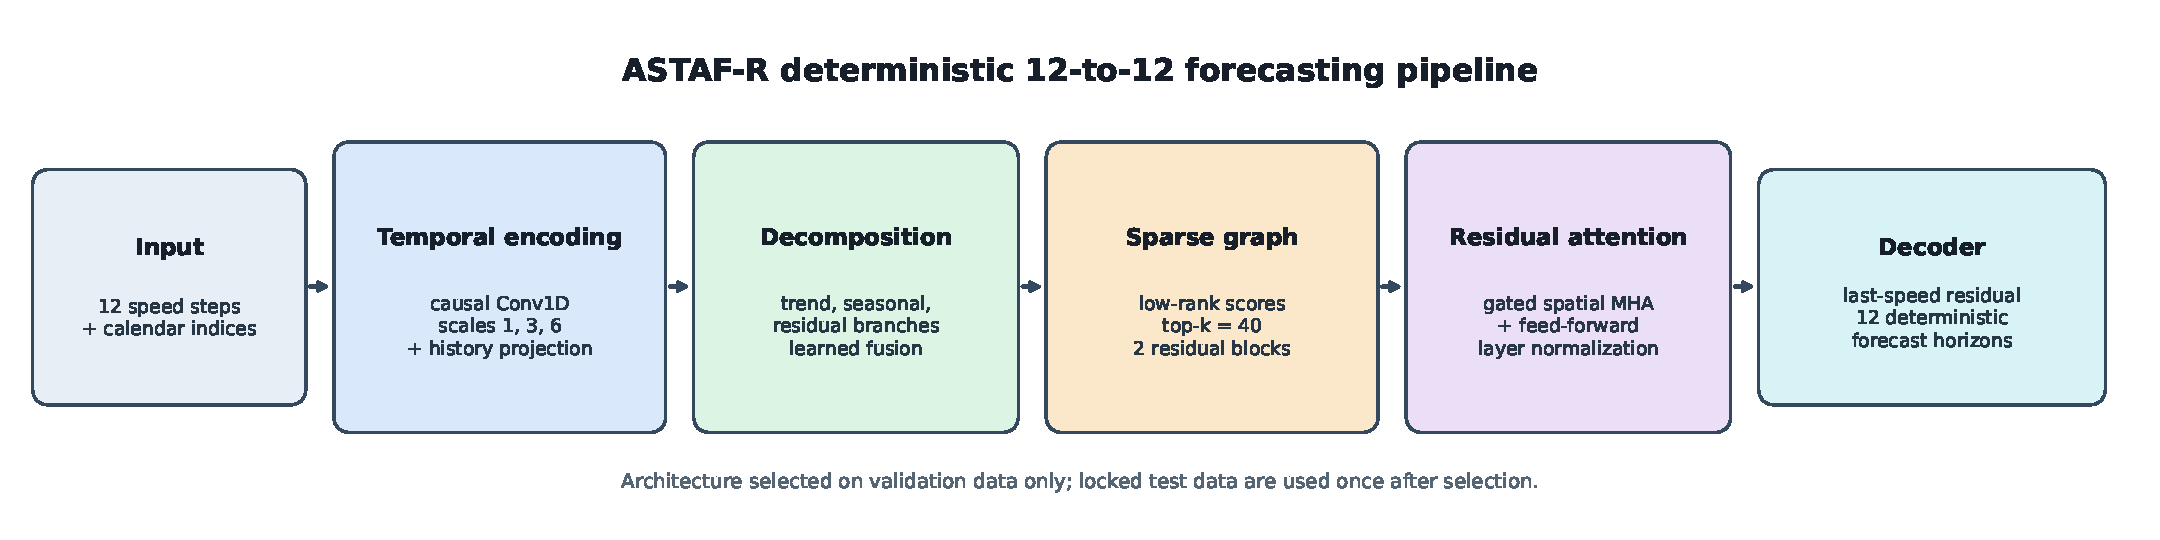
\includegraphics[width=\textwidth]{ASTAFR_round2_architecture.pdf}
\caption{ASTAF-R deterministic forecasting pipeline. The candidate
configuration was selected from validation results before locked testing.}
\label{fig:architecture}
\end{figure*}

\subsection{Causal multi-scale temporal representation}
Parallel one-dimensional convolutions with kernel widths 1, 3, and 6 operate
only on the 12 observed steps. Their outputs are projected to a shared
64-dimensional representation and fused. A separate linear history projection
preserves ordered information from the complete input window. Learned node,
time-of-day, and day-of-week embeddings are added before layer normalization.
All temporal indices are computed from the input-window start; no target value
or future calendar observation enters the encoder.

\subsection{Residual decomposition and learned fusion}
The encoded signal is separated into trend, seasonal, and residual branches.
If their representations are $\mathbf{T}$, $\mathbf{S}$, and $\mathbf{R}$,
the fused representation is
\begin{equation}
\mathbf{H}_{d}=\mathbf{H}_{0}+w_T\mathbf{T}+w_S\mathbf{S}+w_R\mathbf{R},
\end{equation}
where the three non-negative weights are obtained by a softmax and scaled to
the initial total weight. Fixed-weight and decomposition-disabled alternatives
are evaluated on the validation split rather than assumed inferior.

\subsection{Sparse graph propagation}
Two node-embedding matrices $\mathbf{E}_s,\mathbf{E}_t\in\mathbb{R}^{N\times64}$
define directed scores
\begin{equation}
\mathbf{L}=\operatorname{ReLU}\!\left(\mathbf{E}_s\mathbf{E}_t^\top/\sqrt{64}\right)/\tau,
\qquad \tau=0.5.
\end{equation}
Only the largest $k=40$ entries in each row are retained, and a row-wise
softmax produces $\mathbf{A}$. Two residual graph blocks apply
\begin{equation}
\mathbf{H}^{(\ell+1)}=\operatorname{LN}\!\left(\mathbf{H}^{(\ell)}+
\operatorname{Dropout}\left(\mathbf{W}_o\,\operatorname{GELU}
(\mathbf{A}\mathbf{H}^{(\ell)}\mathbf{W}_m)\right)\right).
\end{equation}
Top-$k$, graph depth, reference, shuffled, uniform, identity, and graph-disabled
controls are included in the validation diagnostics.

\subsection{Residual attention and deterministic decoder}
Spatial multi-head attention is applied as a residual update rather than a
mandatory replacement of the graph representation. A feed-forward residual
block and layer normalization follow the attention operation. The decoder maps
each node representation to 12 horizon-specific corrections. These corrections
are added to the last observed speed, providing a strong local reference while
allowing non-persistent forecasts.

\subsection{Loss and optimization}
Training minimizes masked MAE over nonzero targets. Adam uses learning rate
$10^{-3}$, weight decay $10^{-5}$, gradient-norm clipping at 5, mixed precision,
and validation checkpointing. The best validation checkpoint is restored before
the test set is evaluated. The test set is never used for model selection,
epoch selection, or hyperparameter adjustment.

\section{Experimental Setup}
\label{sec:setup}
\subsection{Temporal boundaries and window construction}
Each raw series was divided before window construction. METR-LA used raw index
intervals $[0,23990)$, $[23990,27417)$, and $[27417,34272)$ for training,
validation, and testing. Their timestamp boundaries were 1 March 2012 00:00 to
23 May 2012 07:05, 23 May 2012 07:10 to 4 June 2012 04:40, and 4 June 2012
04:45 to 27 June 2012 23:55. PeMS-BAY used $[0,36473)$, $[36473,41683)$, and
$[41683,52105)$. Windows were then generated independently within each segment,
yielding 23,967/3,404/6,832 METR-LA windows and
36,450/5,188/10,398 PeMS-BAY windows. Thus, the raw-observation intersection
between every pair of splits is empty.

Zero speeds are treated as unavailable. Inputs are mean-imputed after the
training-only global mean and standard deviation are computed; targets retain a
mask so unavailable values do not contribute to loss or metrics. The forecast
horizons are 15, 30, and 60 minutes at steps 3, 6, and 12, in addition to
aggregate 12-step MAE, RMSE, and MAPE.

\subsection{Selection and locked evaluation}
Nine principal candidates were trained with seeds 11, 22, and 33 on both
validation splits. Twenty broader graph, scale, decomposition, context, and
cumulative controls used seed 11. Selection minimized the mean across-dataset
relative validation MAE. The selected two-block, residual-attention,
top-$k=40$ configuration was frozen before any locked-test result was read.
Every learned comparison model was then trained with seeds 11, 22, and 33;
persistence is deterministic and appears once per dataset.

\subsection{Comparison models and reproducibility scope}
The controlled comparison contains compact common-code versions of STID,
DCRNN, STGCN, a Transformer encoder, Graph WaveNet, AGCRN, and the submitted
ASTAF backbone. They share preprocessing, batching, loss, checkpoint selection,
and evaluation code. They are not official checkpoints or exhaustive
method-specific tuning studies, so differences are interpreted only within
this protocol. Runs used Python 3.13.9, PyTorch 2.11.0 with CUDA 12.8, NumPy
2.5.1, and an NVIDIA GeForce RTX 5060 Laptop GPU with 7.96 GiB memory.

\subsection{Statistical and computational analysis}
We report sample mean and sample standard deviation across seeds. Seed-paired
MAE differences are supplemented with exact sign-flip tests; with only three
seeds, the minimum attainable two-sided exact value is 0.25 and is interpreted
accordingly. Prediction windows are also aggregated into non-overlapping
calendar-day blocks. A deterministic 10,000-repetition bootstrap resamples days
within each seed and averages across the three seeds. Computational reporting
includes parameter count, profiler FLOPs, synchronized inference latency, and
peak allocated GPU memory.

\section{Results and Discussion}
\label{sec:results}
\subsection{Validation-only component selection}
Table~\ref{tab:selection} shows the closest principal candidates. The
top-$k=20$ two-block model has slightly lower METR-LA validation MAE than the
selected top-$k=40$ model, whereas top-$k=40$ is lower on PeMS-BAY. The
across-dataset relative criterion selects top-$k=40$ by a narrow margin
(1.000691 versus 1.000794). The one-block model is not selected. Decomposition
disabled, fixed-weight, and learned alternatives are close, so the evidence
does not establish a unique decomposition fusion rule.

\begin{table*}[t]
\centering
\caption{Validation-only evidence for principal architecture choices. Standard
deviations are across seeds 11, 22, and 33.}
\label{tab:selection}
\begin{tabular}{llcc}
\toprule
Dataset & Candidate & Seeds & Validation MAE (mph)\\
\midrule
METR-LA & Fixed decomposition weights & 3 & 2.775$\pm$0.007\\
 & Decomposition disabled & 3 & 2.773$\pm$0.011\\
 & One graph block, top-$k=20$ & 3 & 2.780$\pm$0.008\\
 & No residual output & 3 & 2.785$\pm$0.013\\
 & Two graph blocks, top-$k=20$ & 3 & 2.771$\pm$0.003\\
 & Two graph blocks, top-$k=40$ & 3 & 2.774$\pm$0.006\\
\midrule
PeMS-BAY & Fixed decomposition weights & 3 & 1.571$\pm$0.003\\
 & Decomposition disabled & 3 & 1.577$\pm$0.009\\
 & One graph block, top-$k=20$ & 3 & 1.576$\pm$0.007\\
 & No residual output & 3 & 1.596$\pm$0.009\\
 & Two graph blocks, top-$k=20$ & 3 & 1.574$\pm$0.009\\
 & Two graph blocks, top-$k=40$ & 3 & 1.571$\pm$0.006\\
\bottomrule
\end{tabular}
\end{table*}

\subsection{Locked full-split comparison}
Table~\ref{tab:main_results} reports the locked test results. ASTAF-R has the
lowest mean MAE, RMSE, and MAPE among the compact common-code models on both
datasets. Relative to the strongest MAE comparison, STID-style, its mean MAE is
11.3\% lower on METR-LA and
9.7\% lower on PeMS-BAY. These
numbers support superiority within the declared local pipeline only; they are
not comparisons with official implementations or all published systems.

\begin{table*}[t]
\centering
\caption{Locked-test performance under a common leakage-free protocol. Values
are mean$\pm$sample standard deviation across three seeds, except deterministic
persistence. Lower is better.}
\label{tab:main_results}
\resizebox{\textwidth}{!}{\begin{tabular}{llccc}
\toprule
Dataset & Model & MAE (mph) & RMSE (mph) & MAPE (\%)\\
\midrule
METR-LA & Persistence & 4.286 & 8.214 & 11.167\\
 & STID-style & 3.377$\pm$0.011 & 6.761$\pm$0.018 & 9.931$\pm$0.012\\
 & DCRNN-style & 3.445$\pm$0.007 & 6.813$\pm$0.036 & 9.700$\pm$0.103\\
 & STGCN-style & 5.262$\pm$0.033 & 8.797$\pm$0.060 & 15.203$\pm$0.083\\
 & Transformer-style & 4.460$\pm$0.001 & 9.071$\pm$0.006 & 13.866$\pm$0.025\\
 & Graph WaveNet-style & 3.487$\pm$0.121 & 6.773$\pm$0.280 & 9.878$\pm$0.396\\
 & AGCRN-style & 3.542$\pm$0.192 & 7.022$\pm$0.441 & 10.063$\pm$0.605\\
 & ASTAF backbone & 8.130$\pm$0.003 & 13.347$\pm$0.062 & 27.836$\pm$0.164\\
 & ASTAF-R & \textbf{2.995$\pm$0.008} & \textbf{6.024$\pm$0.010} & \textbf{8.306$\pm$0.024}\\
\midrule
PeMS-BAY & Persistence & 2.170 & 5.123 & 4.671\\
 & STID-style & 1.709$\pm$0.003 & 3.801$\pm$0.002 & 3.945$\pm$0.016\\
 & DCRNN-style & 1.762$\pm$0.003 & 4.018$\pm$0.024 & 4.023$\pm$0.036\\
 & STGCN-style & 3.264$\pm$0.004 & 6.068$\pm$0.013 & 7.617$\pm$0.043\\
 & Transformer-style & 2.489$\pm$0.004 & 5.945$\pm$0.002 & 6.152$\pm$0.046\\
 & Graph WaveNet-style & 1.823$\pm$0.066 & 3.990$\pm$0.204 & 4.196$\pm$0.175\\
 & AGCRN-style & 1.781$\pm$0.091 & 4.045$\pm$0.304 & 4.097$\pm$0.192\\
 & ASTAF backbone & 4.491$\pm$0.001 & 8.803$\pm$0.026 & 12.433$\pm$0.024\\
 & ASTAF-R & \textbf{1.542$\pm$0.001} & \textbf{3.503$\pm$0.009} & \textbf{3.448$\pm$0.025}\\
\bottomrule
\end{tabular}}
\end{table*}

\begin{figure*}[t]
\centering
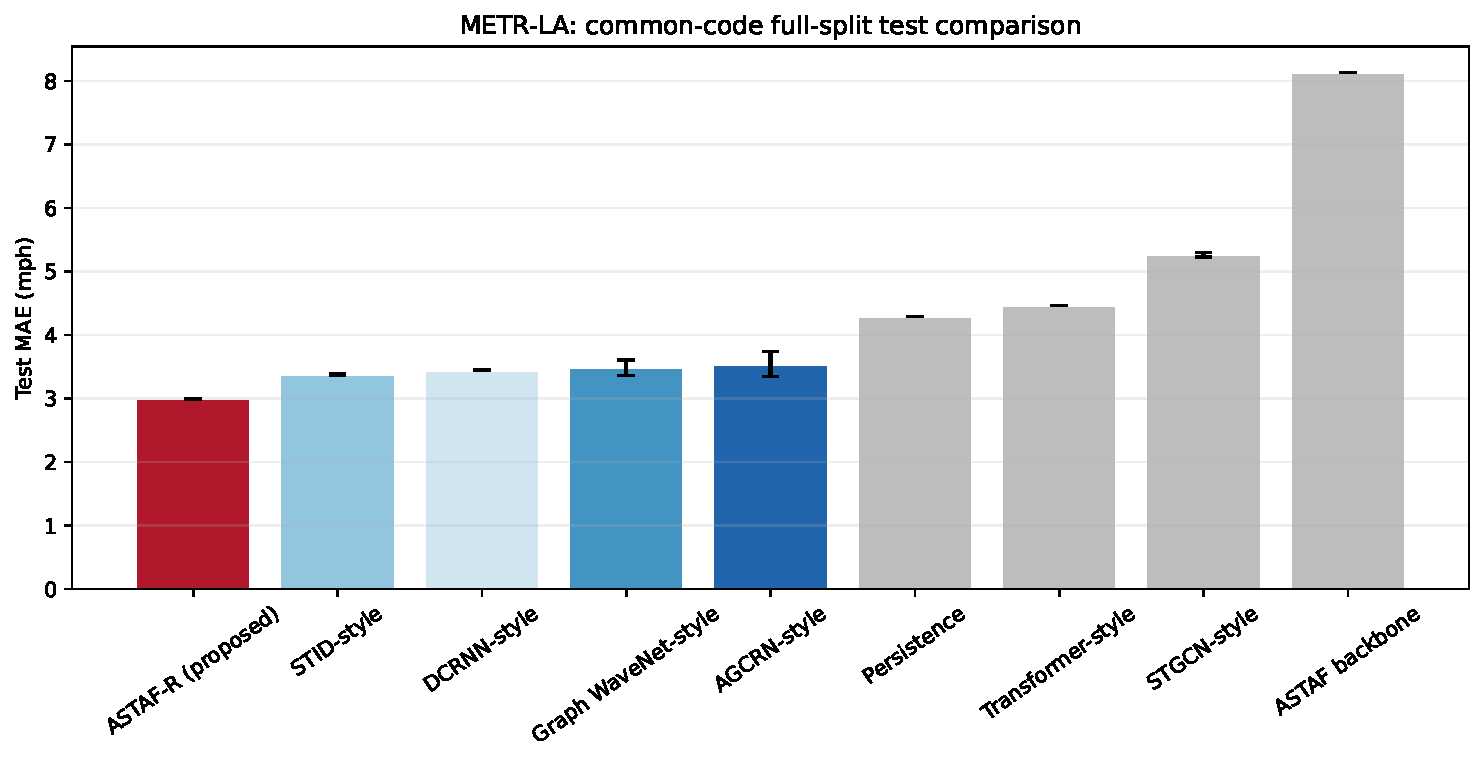
\includegraphics[width=.49\textwidth]{figures/metr_la_mae_comparison.pdf}
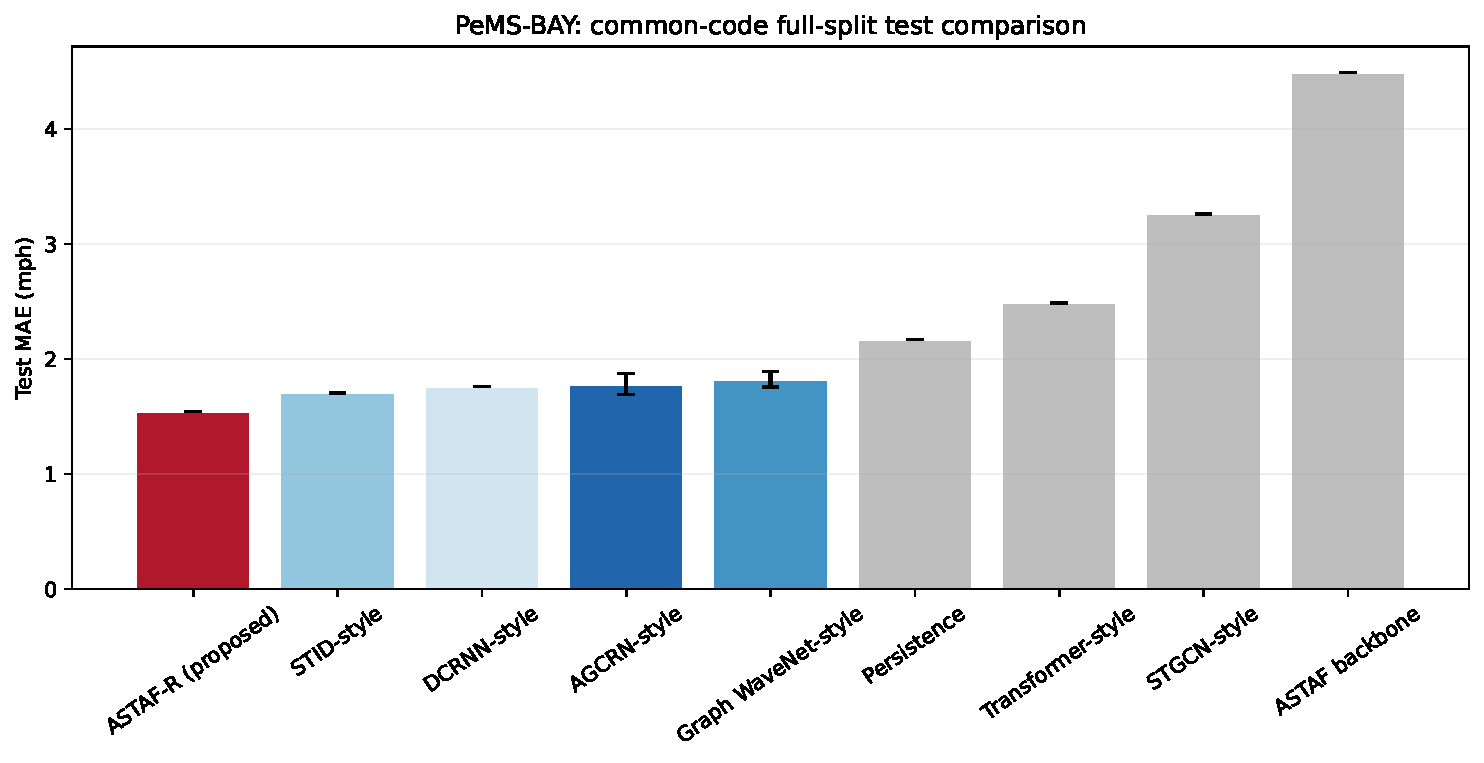
\includegraphics[width=.49\textwidth]{figures/pems_bay_mae_comparison.pdf}
\caption{Locked-test MAE for the compact common-code comparison. Error bars
show sample standard deviation across seeds.}
\label{fig:main_mae}
\end{figure*}

\subsection{Seed and calendar-day variability}
ASTAF-R is lower than every comparison for each matched seed. Exact seed
sign-flip tests remain descriptive because $n=3$ gives low resolution. The
calendar-day block analysis in Table~\ref{tab:statistics} uses 24 METR-LA and
37 PeMS-BAY day blocks per seed. Every 95\% bootstrap interval for ASTAF-R minus
a comparison remains below zero, showing that the aggregate differences are
not driven by a small set of overlapping windows.

\begin{table*}[t]
\centering
\caption{Calendar-day-block MAE differences. Negative values favor ASTAF-R;
intervals are 10,000-repetition clustered day-bootstrap intervals.}
\label{tab:statistics}
\resizebox{\textwidth}{!}{\begin{tabular}{llccc}
\toprule
Dataset & Comparison & Mean difference & 95\% block CI & Seed SD\\
\midrule
METR-LA & vs. AGCRN-style & -0.520 & [-0.573, -0.470] & 0.174\\
 & vs. ASTAF backbone & -4.751 & [-5.057, -4.425] & 0.008\\
 & vs. DCRNN-style & -0.429 & [-0.461, -0.397] & 0.011\\
 & vs. Graph WaveNet-style & -0.467 & [-0.507, -0.428] & 0.109\\
 & vs. STGCN-style & -2.104 & [-2.221, -1.981] & 0.028\\
 & vs. STID-style & -0.363 & [-0.395, -0.332] & 0.009\\
 & vs. Transformer-style & -1.362 & [-1.490, -1.227] & 0.006\\
\midrule
PeMS-BAY & vs. AGCRN-style & -0.236 & [-0.262, -0.209] & 0.090\\
 & vs. ASTAF backbone & -2.904 & [-3.103, -2.707] & 0.001\\
 & vs. DCRNN-style & -0.218 & [-0.239, -0.196] & 0.003\\
 & vs. Graph WaveNet-style & -0.278 & [-0.304, -0.251] & 0.065\\
 & vs. STGCN-style & -1.701 & [-1.783, -1.617] & 0.004\\
 & vs. STID-style & -0.164 & [-0.180, -0.148] & 0.004\\
 & vs. Transformer-style & -0.931 & [-1.036, -0.825] & 0.005\\
\bottomrule
\end{tabular}}
\end{table*}

\subsection{Graph diagnostic}
\label{subsec:graph_robustness}
The cross-seed adjacency correlation and top-20 Jaccard values are exactly one
to numerical precision (Table~\ref{tab:graph_stability}). Inspection of the
six restored best checkpoints explains this result: both graph-embedding
matrices have zero norm, all pre-softmax graph logits are zero, and deterministic
top-$k$ tie handling selects the same 40 indices per row. Each selected edge
therefore has weight $1/40=0.025$. This is a degenerate uniform sparse graph,
not evidence that independently initialized adaptive topologies converged to a
stable road-network structure. The correct conclusion is that sparse graph
averaging is compatible with the selected model; learned-topology recovery is
not validated by these runs.

\begin{table}[t]
\centering
\caption{Cross-seed graph diagnostics reported without rounding away the exact
identity. The identity is explained by zero graph embeddings and uniform
top-40 weights.}
\label{tab:graph_stability}
\resizebox{\columnwidth}{!}{\begin{tabular}{lccc}
\toprule
Dataset & Seed pair & Pearson correlation & Top-20 Jaccard\\
\midrule
METR-LA & 11--22 & 1.000000000000 & 1.000000000000\\
METR-LA & 11--33 & 1.000000000000 & 1.000000000000\\
METR-LA & 22--33 & 1.000000000000 & 1.000000000000\\
PeMS-BAY & 11--22 & 1.000000000000 & 1.000000000000\\
PeMS-BAY & 11--33 & 1.000000000000 & 1.000000000000\\
PeMS-BAY & 22--33 & 1.000000000000 & 1.000000000000\\
\bottomrule
\end{tabular}}
\end{table}

\begin{figure}[t]
\centering
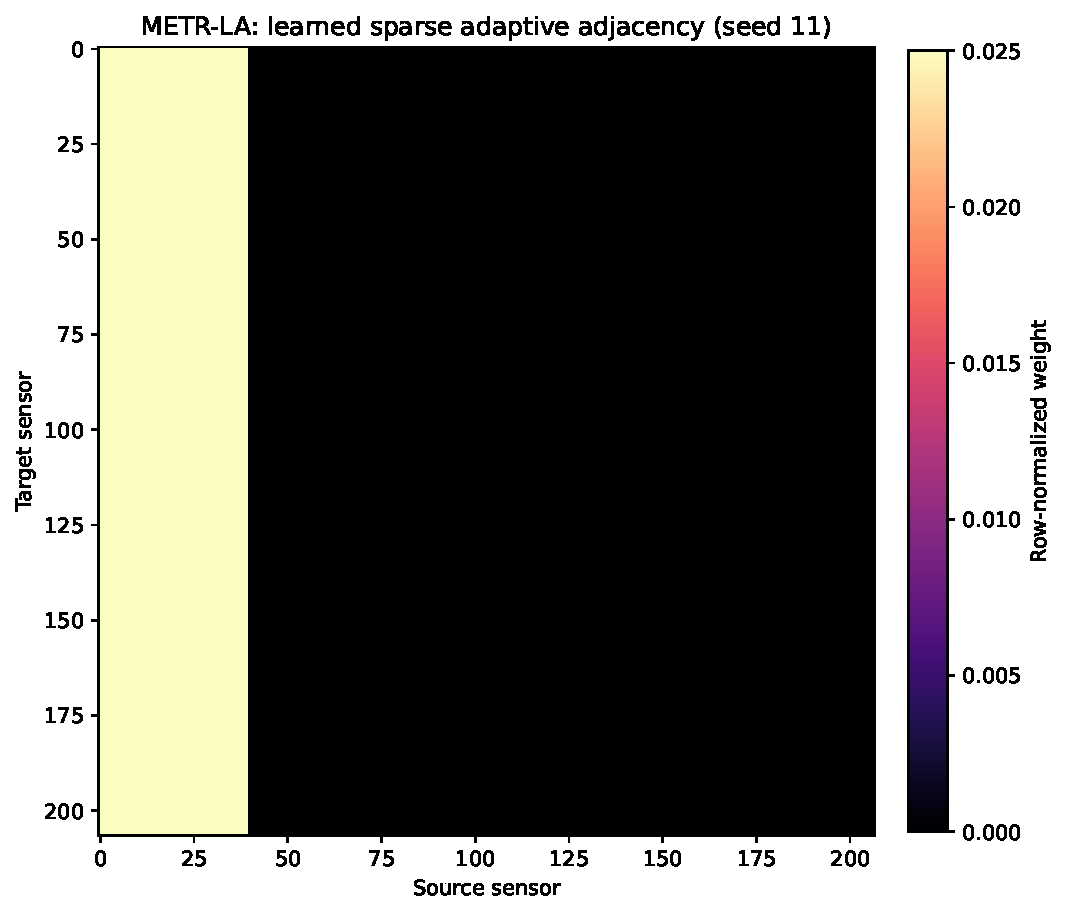
\includegraphics[width=\columnwidth]{figures/metr_la_learned_adjacency.pdf}
\caption{METR-LA sparse graph matrix from seed 11. The uniform nonzero weights
and deterministic support must not be interpreted as recovered topology.}
\label{fig:graph}
\end{figure}

\subsection{Forecast horizons and engineering trade-offs}
Error increases with horizon on both datasets (Figure~\ref{fig:horizon}),
while ASTAF-R retains the lowest mean MAE in the local comparison at all 12
horizons. The accuracy comes with higher parameter count and greater inference
memory/latency than STID-, DCRNN-, and STGCN-style controls
(Table~\ref{tab:efficiency}). ASTAF-R is therefore not the preferred choice
when minimum memory or latency dominates accuracy; deployment selection should
use the application-specific trade-off.

\begin{figure*}[t]
\centering
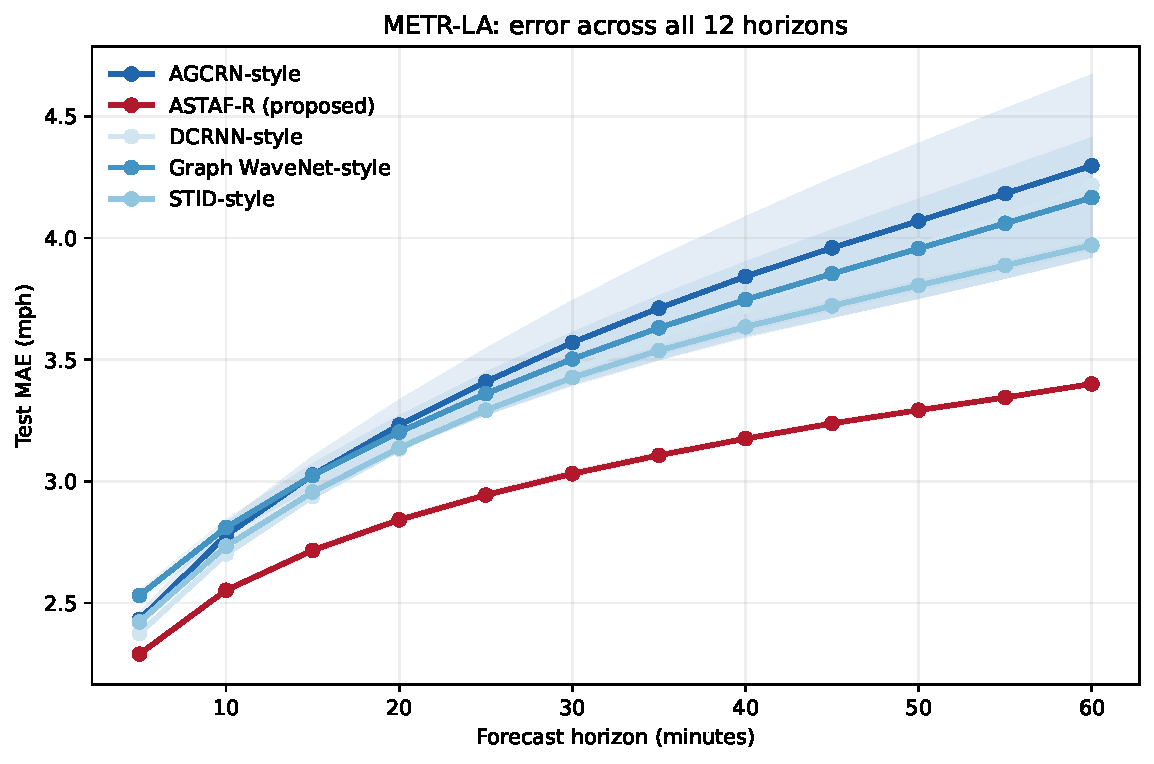
\includegraphics[width=.49\textwidth]{figures/metr_la_horizon_mae.pdf}
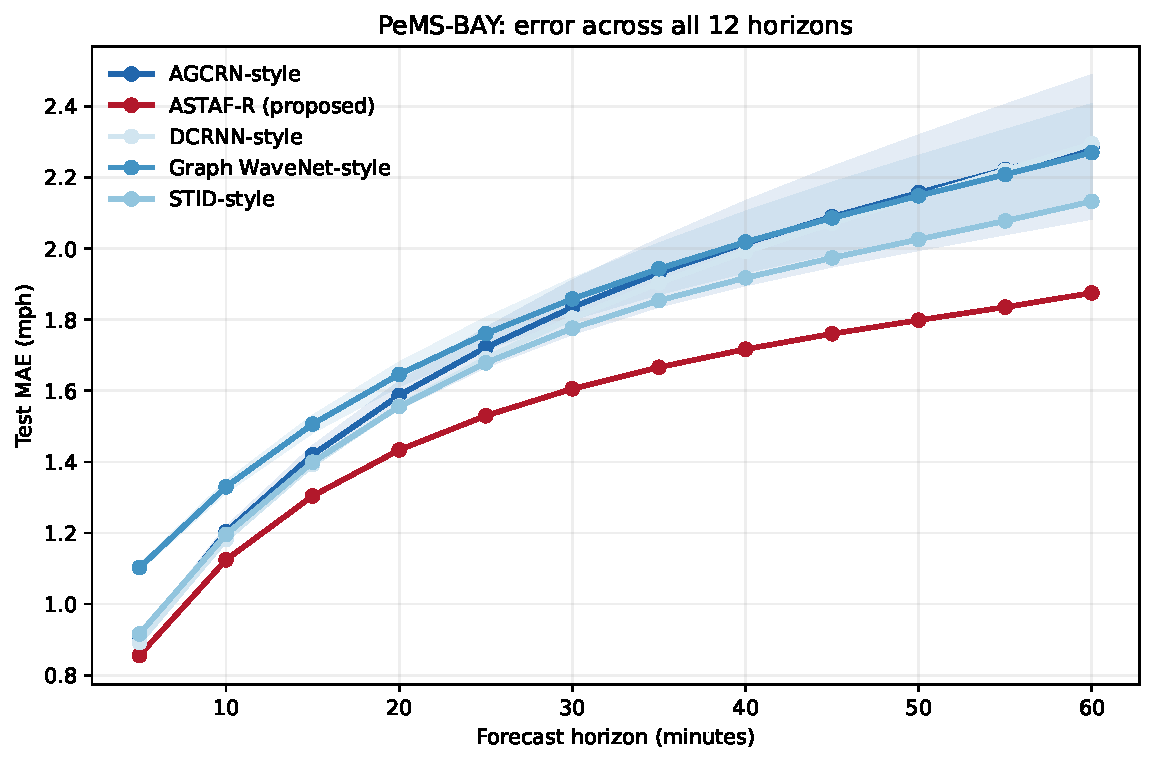
\includegraphics[width=.49\textwidth]{figures/pems_bay_horizon_mae.pdf}
\caption{MAE across the 12 five-minute forecast horizons. Shading denotes
sample standard deviation across seeds.}
\label{fig:horizon}
\end{figure*}

\begin{table*}[t]
\centering
\caption{Environment-specific computational profile. Latency and peak memory
are not hardware-independent model properties.}
\label{tab:efficiency}
\resizebox{\textwidth}{!}{\begin{tabular}{llrrrr}
\toprule
Dataset & Model & Parameters & FLOPs & Latency (ms/sample) & Peak GPU (MiB)\\
\midrule
METR-LA & ASTAF-R & 133,842 & 52,053,945 & 0.184 & 377.9\\
 & STID-style & 38,028 & 2,358,209 & 0.017 & 28.8\\
 & DCRNN-style & 38,412 & 454,333,536 & 0.233 & 48.9\\
 & Graph WaveNet-style & 114,765 & 1,344,774,051 & 0.253 & 303.9\\
 & AGCRN-style & 60,493 & 896,704,128 & 0.200 & 55.4\\
 & Persistence & 0 & -- & 0.001 & 18.5\\
 & Transformer-style & 100,876 & 341,480,448 & 0.430 & 412.9\\
 & STGCN-style & 13,516 & 193,950,720 & 0.051 & 115.8\\
 & ASTAF backbone & 91,984 & 752,433,408 & 0.193 & 377.0\\
\midrule
PeMS-BAY & ASTAF-R & 156,498 & 106,271,169 & 0.312 & 578.2\\
 & STID-style & 45,580 & 3,702,465 & 0.028 & 33.8\\
 & DCRNN-style & 38,412 & 952,629,600 & 0.385 & 66.1\\
 & AGCRN-style & 75,597 & 2,100,009,600 & 0.217 & 109.1\\
 & Graph WaveNet-style & 129,869 & 2,921,427,275 & 0.423 & 467.1\\
 & Persistence & 0 & -- & 0.002 & 19.2\\
 & Transformer-style & 100,876 & 536,140,800 & 0.686 & 637.0\\
 & STGCN-style & 13,516 & 422,323,200 & 0.095 & 171.1\\
 & ASTAF backbone & 107,088 & 1,839,136,000 & 0.358 & 576.5\\
\bottomrule
\end{tabular}}
\end{table*}

\subsection{Scope of the evidence}
The experiments cover two California freeway-speed datasets with regular
five-minute sampling and no exogenous weather, event, or incident variables.
They do not establish transfer to other cities, irregular sampling, flow or
occupancy targets, distribution shift, or heterogeneous multi-frequency
covariates. The deterministic evaluation also does not establish calibrated
uncertainty forecasting.

\section{Conclusion and Future Work}
\label{sec:conclusion}
ASTAF-R was evaluated using validation-only architecture selection and a locked,
leakage-free test protocol on METR-LA and PeMS-BAY. It achieved the lowest mean
error among the compact common-code controls on both datasets, with small
between-seed dispersion and calendar-day bootstrap intervals favoring ASTAF-R.
The conclusion is deliberately protocol-specific: official baseline
implementations were not executed, and two California freeway datasets cannot
support a universal generality claim.

The diagnostic evidence also changes the interpretation of the graph module.
The graph embeddings converged to zero, producing an identical uniform top-40
support across seeds. The present results therefore support sparse graph
propagation as part of the forecasting computation, but they do not validate
adaptive topology recovery. Similarly, closely matched decomposition variants
do not identify one fusion rule as uniquely effective.

Future work should compare official baseline repositories under harmonized
splits, repair or regularize the graph learner to avoid zero-embedding collapse,
repeat selection after that change, and evaluate geographically distinct and
irregularly sampled networks with exogenous variables. Probabilistic extensions
should be trained with proper scoring rules and evaluated using coverage,
interval width, calibration error, and distributional scores.

\section{Reproducibility Record}
The public archive contains preprocessing, model, training, evaluation, and
baseline code; configuration values; random seeds; environment dependencies;
run-level JSON and NumPy artifacts; generated analysis tables; and commands for
reproducing the study. Exact raw-split boundaries and the absence of
cross-split raw-observation overlap are recorded in every locked-test run.

\section*{Author contributions statement}

S.S. Chauhan conceived the study, contributed to the research design, and led the initial manuscript preparation.
P. Nema contributed to data preprocessing, model implementation, and experimental execution.
G. Chhabra assisted in methodological refinement, validation, and interpretation of the experimental results.
A. Pandey supervised the study, contributed to result analysis, visualization, critical manuscript revision, and coordinated the final submission.
S. Syal contributed to literature analysis, manuscript editing, and interpretation of the findings.
All authors reviewed the manuscript, provided intellectual input, approved the final version, and agreed to be accountable for the content of the work.
Correspondence should be addressed to A. Pandey.

\section*{Competing interests}

The authors declare no competing interests.

\section*{Funding Declaration}

The authors received no specific funding for this work.

\section*{Data Availability}
METR-LA and PeMS-BAY are publicly available from the Zenodo dataset releases
at \url{https://doi.org/10.5281/zenodo.5724362} and
\url{https://doi.org/10.5281/zenodo.5146275}.

\section*{Code Availability}
The complete source code, preprocessing, model and compact baseline
implementations, configuration values, dependencies, seeds, training and
evaluation commands, and analysis scripts are publicly available at
\url{https://github.com/shishirbit/ASTAF-R-reproducibility}. The exact version used for this article will be archived at
Zenodo under \texttt{ZENODO-DOI-PENDING-VERSIONED-RELEASE}; this placeholder will be replaced
with the minted DOI before submission.

\bibliography{reference}

\end{document}
